%%
%% Тема практики: <<Автоматизированная разработка программно-аппаратного комплекса
%% ''цифровые часы с будильником'' на базе микроконтроллера AVR семейства XMega>>
%%
\documentclass[russian,simple,utf8,pointsubsection,reduceheight=20mm]{eskdtext}
\usepackage[utf8]{inputenc}
\usepackage[russian]{babel}
\usepackage{ucs}
\usepackage[unicode]{hyperref}
\usepackage{multirow}
\usepackage{amstext}
\usepackage{amsmath}
\usepackage{listings}
\graphicspath{{/Users/zolkko/Projects/zolkko-alarm/doc/imgs/}}
\usepackage{longtable}
\usepackage{geometry}



\ESKDdepartment{}
\ESKDcompany{}
\ESKDclassCode{31 1398}
\ESKDdocName{Пояснительная записка}
\ESKDsignature{Автоматизированная разработка программно-аппаратного комплекса на базе микроконтроллера AVR семейства XMega}
\ESKDtitle{Отчёт по преддипломной практике}
\ESKDauthor{Анисимов~А.~Н.}
\ESKDtitleApprovedBy{Руководитель}{Барабанов~В.~Ф.}
\ESKDtitleAgreedBy{Руководитель}{Барабанов~В.~Ф.}
\ESKDtitleDesignedBy{студент группы ВМ-072}{Анисимов А.Н.}

%% первая страница и титульный лист без рамок и кастомный формат
\ESKDdefaultTitleStyle{empty}
\ESKDdefaultFirstStyle{empty}
\ESKDdefaultStyle{empty}

%% Уменьшаю размер шрифта колонки №1 основной надписи, так что бы эта
%% "умная" дура всё таки влезла в рамку
\renewcommand{\ESKDfontVIIsize}{\fontsize{10pt}{12pt}}

%% пол умалчанию перечисления используют арабские цифры
\renewcommand{\theenumi}{\arabic{enumi}}

%% Сказали, что в перечислених ни каких булетов не должно быть
\renewcommand{\labelitemi}{}
\renewcommand{\labelitemii}{}
\renewcommand{\labelitemiii}{}
\renewcommand{\labelitemiv}{}

%% Главные заголовки центрируються
\renewcommand{\ESKDsectionAlign}{\ESKDsectAlignCenter}
\renewcommand{\ESKDsectionStyle}{\normalfont\MakeUppercase}
\renewcommand{\ESKDsubsectionStyle}{\normalfont}
\renewcommand{\ESKDsubsubsectionStyle}{\normalfont}

%% \renewcommand{\bibname}{Test}


\geometry{left=20mm}
\geometry{right=20mm}
\setlength{\footskip}{0mm}


\begin{document}
\pagestyle{plain}
\thispagestyle{empty}
\begin{center}
Федеральное агентство по образованию \\*
ГОСУДАРСТВЕНОЕ ОБРАЗОВАТЕЛЬНОЕ УЧРЕЖДЕНИЕ \\*
ВЫСШЕГО ПРОФЕССИОНАЛЬНОГО ОБРАЗОВАНИЯ \\*
<<ВОРОНЕЖСКИЙ ГОСУДАРСТВЕННЫЙ ТЕХНИЧЕСКИЙ УНИВЕРСИТЕТ>> \\
\end{center}
\begin{center}
Факультет  автоматики и электромеханики \\
\end{center}
\begin{center}
Кафедра автоматизированных и вычислительных систем \\
\end{center}

\begin{center}
Специальность 230101 <<Вычислительные машины, комплексы, системы и сети>>
\end{center}

\vspace{1em}

\begin{center}
ОТЧЁТ \\*
ПО ПРЕДДИПЛОМНОЙ ПРАКТИКЕ \\*
Тема практики: <<Автоматизированная разработка программно-аппаратного комплекса
''цифровые часы с будильником'' на базе микроконтроллера AVR семейства XMega>>
\end{center}

\vspace{1em}

\begin{tabular}{p{12em}p{5em}@{}p{5em}@{}r@{}r}
Выполнил студент группы & \hrulefill{} ВМ-072 & \hrulefill{}  & \hrulefill{} А.Н. Анисимов \\
 &  \small{Группа}  & \small{Подпись} &\small{Инициалы, фамилия} \\
& & & \\
\multirow{2}{12em}{Руководитель практики\newline{} от кафедры АВС} & \hrulefill{} & \hrulefill{} & \hrulefill{} О. Я. Кравец \\
 & \small{Подпись}  & \small{Дата} & \small{Инициалы, фамилия} \\
 & & & \\
\multirow{2}{12em}{Руководитель дипломного  проекта} & \hrulefill{} & \hrulefill{} & \hrulefill{} А. В. Барабанов \\
 & \small{Подпись}  & \small{Дата} & \small{Инициалы, фамилия} \\
& & & \\
\multirow{2}{12em}{Консультант дипломного проекта} & \hrulefill{} & \hrulefill{} & \hrulefill{} В.Ф. Барабанов \\
 & \small{Подпись}  & \small{Дата} & \small{Инициалы, фамилия} \\
& & & \\
\multirow{2}{12em}{Руководитель по экономической части} & \hrulefill{} & \hrulefill{} & \hrulefill{} Т.С. Наролина \\
 & \small{Подпись}  & \small{Дата} & \small{Инициалы, фамилия} \\
& & & \\
Защищена \hrulefill{} &  & Оценка \hrulefill{} & \hrulefill{} 
\end{tabular}

\vspace{1.5em}

\begin{center}
г. Воронеж \\*
2011 г.
\end{center}

\newpage

\setlength{\footskip}{10mm}

\renewcommand{\contentsname}{СОДЕРЖАНИЕ}

\begin{center}
\MakeUppercase{ЗАМЕЧАНИЯ РУКОВОДИТЕЛЯ}
\end{center}
\newpage

%% В ВГТУ по какой-то причине не считаются с существованием ЕСКД
%\ESKDthisStyle{formI}
%\setcounter{page}{3}
\tableofcontents
\newpage

%% Введение
%!TEX root = /Users/zolkko/Projects/zolkko-alarm/doc/main.tex
\section*{Введение}
\addcontentsline{toc}{section}{Введение}
\begin{par}
На сегодняшний день при проектировании систем промышленной автоматизации и устройств
бытового применения, перед проектировщиками и разработчиками встают вопросы не только технического
характера, но и вопросы экономической целесообразности применения тех или иных решений.
То есть при их решении необходимо учитывать не только системные характеристики применяемых для
реализации конечных устройств технологий, но и искать компромис с их стоимостью. При этом
на конечную стоимость изделия будут влиять цена применённых схемотехнических решений,
время затраченное на проектирование и реализацию устройства, цена применяемых средства автоматизации
и цена специалистов проектировщиков и разработчиков.
\end{par}

\begin{par}
Немаловажным при проектировании устройств является учёт стремления
современной европейской культуры не только к открытым, но и полностью свободным системам,
зачастую обладающим более качественными системными и
потребительскими характеристиками и способствующими общему\\*
научно-техническому прогрессу \cite{lessing}.
\end{par}


В дипломном проекте рассмотрены современные методы и средства проектирования и разработки
программно-аппаратным комплексов на базе микроконтроллеров AVR компании Ateml. При этом
в процессе проектирования и разработки отдавалось предпочтение именно свободному или
доступному по цене программному и аппаратному обеспечению. В качестве примера разрабатывался
программно-аппаратный комплекс <<Универсальная система терморегулирования на базе
микроконтроллера AVR cемейства XMega>>. Таким образом в процессе выполнения дипломного проекта
стало возможным проведение анализа пригодности для практического применения свободного,
бесплатного и доступного по цене программного и аппаратного обеспечения для целей промышленного
производства.

Программный код написанный в процессе выполнения дипломного проекта использует большинство
внешней периферии микроконтроллера. Таким образом, сформированный программный код и электрическая
принципиальная схема, позволяют оценить преимущества и недостатки использования
микроконтроллеров AVR семейства XMega.

\newpage{}



%% Постановка задачи
\section{Постановка задачи}
\begin{par}
Спроектировать и разработать устройство позволяющее в заданные моменты времени выдавать сигнал
звукового оповещения, производить индикацию текущего времени, а так же прозводить его синхронизацию
с удалённым сервером используя вычислительную сеть стандарта 802.3 Ethernet.
\end{par}

\begin{par}
Центральный вычислительный модуль устройства должен быть выполнен на микроконтроллере AVR компании
Atmel семейства XMega.
\end{par}

\begin{par}
Не смотря на то, что реализация подобного устройства на ПЛИС имеет ряд преимуществ по
сравнению с реализацией на основе микроконтроллеров, а именно более высокая скорость
работы и более низкое потребление энергии, новое семейство 8-битных микроконтроллеров
AVR переносит микроконтроллерные устройства на новый уровень системных характеристик,
которые в сочетации с более низкой стоимостью самих микроконтроллеров и иструментария
разработчика, делает их адекватным выбором при проектировании систем. Микроконтроллеры
AVR семейства XMega интегрируют в себе устройства ввода-вывода с улучшенными характеристиками,
более низкую потребляемую мощьность за счёт применения в них новой технологии picoPower.
Новая система обработки событий Event System, обеспечивает независимую от ЦПУ
быстродействующую передачу данных между внутренними переферийными устройствами 4-канального
контроллера ПДП, улучьшающего характеристики микроконтроллера. Микроконтроллеры имеют
быстродействующие 12-битнее модули АЦП и ЦАП. И ускоритель криптографических алгоритмов AES и DES.
Каждое перечисленное нововведение в семействе XMega микроконтроллеров AVR, позволит
в более сжатые сроки, а следовательно и с меньшими финансовыми затратами реализовать
целевое устройство, при этом отставание в производительности и потребляемой мощьности
становиться не значительным для данного класса устройств.
\end{par}

\begin{par}
Необходимо в качестве устройств ввода и вывода использовать один модуль сенсорного экрана
для уменьшения рабочей поверхности изделия.
\end{par}

\begin{par}
В качестве устройства взаимодействия с удалённым сетевым сервисом времени необходимо использовать
контроллер фирмы Micro Chip enc28j60. Применени этого контроллера позволит устройству производить
синхронизацию текущего времени по протоколу SNTP.
\end{par}

\begin{par}
Необходимо споектировать и разработать:
    \begin{itemize}
        \item{}Принципиальную электрическую схему;
        \item{}печатную плату.
    \end{itemize}
\end{par}

\begin{par}
Необходимо разработать на языке высокого уровня С++  программу управления устройва:
\begin{itemize}
    \item{} Модуль учёта текущего времени;
    \item{} модуль индикации текущего времени, выводящий информацию о текущем времени на ЖК-дисплее;
    \item{} модуль пользовательского ввода с сенсорного экрана, обеспечивающий первоначальную
            конфигурацию устройства, и установку времени срабатывания звукового сигнала;
    \item{} модуль воспроизведения звукового сигнала с внешней энергонезависимой памяти;
    \item{} модуль синхронизации текущего времени с удалённым SNTP сервисом.
\end{itemize}
\end{par}
\newpage{}


%% Обзор САПР
%!TEX root = /Users/zolkko/Projects/zolkko-alarm/doc/main.tex
\section{Анализ современных систем автоматизированного проектирования про\-гра\-ммно\--аппа\-ра\-тных микроконтроллерных комплексов}

\subsection{Общие сведения о САПР}
\begin{par}
САПР --- Система автоматизированного проектирования --- автоматизированная система, реализующая
информационную технологию выполнения функций проектирования, представляет собой
организационно-техническую систему, предназначенную для автоматизации процесса проектирования,
состоящую из персонала и комплекса технических, программных и других средств
автоматизации его деятельности.
\end{par}

\begin{par}
На некотором этапе своего развития системы проектирования претерпели качественное изменение.
Оно было связано с тем, что САПР из набора каким-то образом связанных между собой прикладных
программ начали превращаться в мобильные и стройно организованные системы, способные к
настройке на особенности предметной области и на требования конечного пользователя,
допускающие расширение функциональных возможностей за счёт сравнительно несложного подключения
новых прикладных программных модулей и обеспечивающих поддержку групповой разработки сложных схем
коллективом проектировщиков.
\end{par}

\begin{par}
Особенное значение САПР приобрели в микроэлектронике, поскольку современная радиоэлектронная аппаратура базируется на применении сверхбольших
интегральных схем, разработка которых без применения САПР невозможна или крайне затруднительна.
\end{par}

\begin{par}
Специализированные САПР для разработки электронных устройств и печатных плат получили название
Electronic Design Automation - EDA, автоматизация проектирования электронных приборов.
Комплексы такого типа зачастую позволяют создавать принципиальные электрические схемы схемы с
помощью графического интерфейса, создавать и модифицировать  базу радиоэлектронных компонентов,
проверять целостность сигналов на ней и проводить аналоговое и цифровое моделирование
разрабатываемого устройства ещё на этапе проектирования.
\end{par}


\subsubsection{Обзор Electric VLSI}
\begin{par}
Electric VLSI --- cистема автоматизированного проектирования сверхбольших интегральных схем, используемая для разработки электрических схем и проектирования
топологии печатных плат и интегральных схем.
\end{par}
\begin{par}
Electric являлся open-source проектом, разработка
которого в течении многих лет поддерживалась\cite{electric} компанией Sun Microsystems,
а в настоящее время курируется компанией Oracle. \\*
Наиболее ценная встроенная в Electric возможность —-- это система привязок,
которая даёт возможность осуществлять проектирование сверху вниз с соблюдением целостности
всех соединений.
\end{par}

\subsubsection{Обзор Proteus VSM}
\begin{par}
Proteus VSM --- пакет программ для автоматизированного проектирования электронных схем.
    Разработка компании Labcenter Electronics.
\end{par}
\begin{par}
Proteus VSM сочитает в себе функциональность SPICE симуляции электронных цепей,
анимированные компоненты, модели микропроцессоров и средства симуляции сложных
микроконтроллерых решений. Это первая система сочетающая в себе все эти особенности
и позволяющая разработать и протестировать решение до создания прототипа устройства.
Такое тестирование осуществляется за счёт взаимодействия с отображаемыми и анимированными
виртуальными устройствами такими как свето-диоды, LCD, кнопки и переключатели.
При этом симуляция производится в режиме блиском к режиму реального времени.
Так производительности 1 ГГц Pentium III ЭВМ будет достаточно для симуляции работы
микропроцессора 8051 на частоте 12 МГц в режиме реального времени. Так же Proteus VSM
предоставляет экстенсивные средства отладки, включая точки останова, трассировку и вывод
значений  переменных микропрограмм как для машинных кодов, так и для языков высокого
уровня. Proteus VSM  включает несколько виртуальныхинструментов: осцилограф, логический
анализатор, генератор функций, генератор по шаблонам, виртуальный терминал, отладчики SPI
и I2C интерфейсов , а так же простые инструменты как вольтметр и амперметр, существенно
облегчающих анализ и отладку схемы.
\end{par}
\begin{par}
В дополнении к моделям микропроцессоров в Proteus VSM так же включена большая библиотека
стандартных пассивных и акивных моделей устройств.
\end{par}
\begin{par}
Пакет Proteus состоит из двух частей, двух подпрограмм: ISIS – программа синтеза и
моделирования непосредственно электронных схем и ARES – программа разработки печатных
плат.

\begin{figure}[h]
	\center{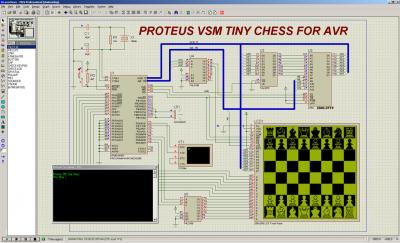
\includegraphics[bb=0 0 400 243, clip, scale=0.8]{proteus.png}}
	\caption{Главное окно программы Proteus ISIS}
	\label{img:proteus}
\end{figure}

\end{par}

\subsubsection{Обзор KiCAD}
\begin{par}
KiCad --- распространяемый по лицензии GNU General Public License программный
комплекс класса EDA с открытыми исходными текстами, предназначенный для разработки
электрических схем и печатных плат. \\*
Кроссплатформенность компонентов KiCad обеспечивается использованием библиотеки wxWidgets.
Поддерживаются операционные системы Linux, Windows NT 5.x, FreeBSD и Solaris.
\begin{figure}[h]
	\center{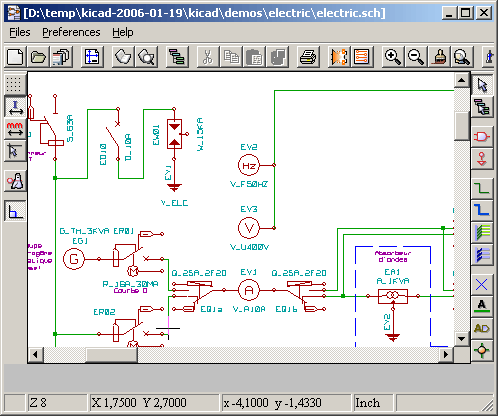
\includegraphics[bb=0 0 498 416, clip, scale=0.5]{kicad.png}}
	\caption{Главное окно программы KiCAD Eeschema}
	\label{img:kicad}
\end{figure}
\end{par}

\begin{par}
В состав KiCAD входят программы:
    \begin{itemize}
        \item{}kicad --— менеджер проектов;
        \item{}eeschema —-- редактор электрических схем (рис. \ref{img:kicad});
        \item{}встроенный редактор символов схем (библиотечных компонентов);
        \item{}pcbnew --— редактор печатных плат;
        \item{}встроенный редактор образов посадочных мест (библиотечных компонентов);
        \item{}3D Viewer --— 3D-просмотрщик печатных плат на базе OpenGL (часть pcbnew);
        \item{}gerbview --— просмотрщик файлов Gerber (фотошаблонов);
        \item{}cvpcb --— программа для выбора посадочных мест, соответствующих компонентам на схеме;
        \item{}wyoeditor --— текстовый редактор для просмотра отчетов.
    \end{itemize}
\end{par}


\subsubsection{Обзор gEDA}
\begin{par}
gEDA --- набор программного обеспечения для проектирования электронных устройств,
распространяемый по лицензии GPL. Включает в себя инструменты для редактирования
электрических схем, симуляции цифровых и аналоговых схем, трассировки печатных плат
и подготовки к производству. Проект изначально ориентирован на UNIX-совместимые
платформы, хотя некоторые программы, входящие в его состав, в настоящее время
портированы под ОС Windows\cite{geda}.
\end{par}
\begin{par}
В настоящее время пакет вполне пригоден для проектирования устройств среднего уровня
сложности и может быть полезен как студентам, любителям, так и профессиональным
разработчикам электронных устройств.
\end{par}
\begin{par}
За время существования проекта, к нему примкнуло несколько самостоятельных
узкоспециализированных проектов, которые теперь считаются частью gEDA, в
связи с чем оригинальный проект и его составные части стали называть
gEDA/gaf (gschem and friends) (рис. \ref{img:geda}).
\begin{figure}[h]
	\center{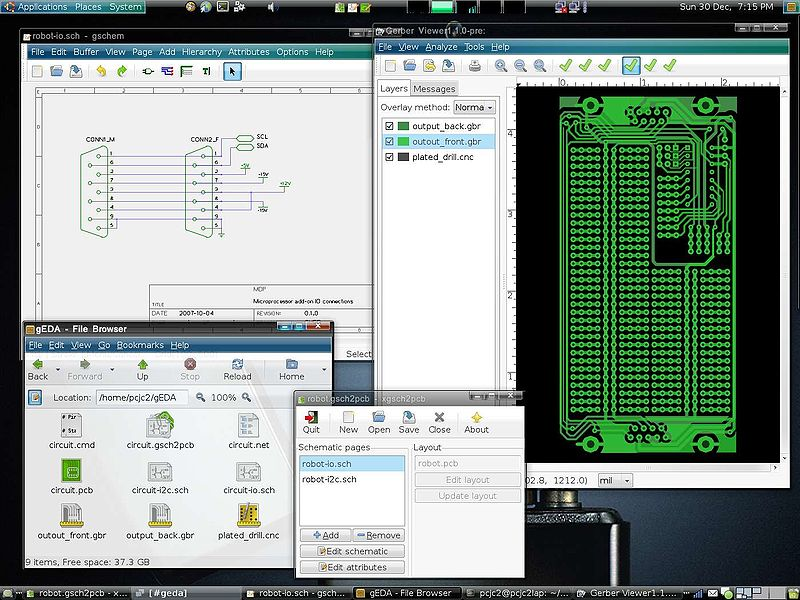
\includegraphics[bb=0 0 800 600, clip, scale=0.3]{geda.png}}
	\caption{gEDA}
	\label{img:geda}
\end{figure}
\end{par}

\subsubsection{Обзор Eagle EDA}
\begin{par}
EAGLE это лёгкий в использовании, но достаточной мощный EDA пакет, разрабатываемый немецкой компанией CadSoft.
В состам системы входят:
\begin{enumerate}
	\item{}Layout Editor --- пограмма для проектирования печатных плат (рис. \ref{img:eagle_brd}). 
		\begin{itemize}
			\item{}Максимальная рабочая поверхность 1.6 x 1.6м;
			\item{}разрешение - 1/10,000мм (0.1 микрон);
			\item{}до шестнадцати сигнальных слоёв;
			\item{}большая библиотека компонентов;
			\item{}copper pouring - области на печатной плате заполненные  медью, что часто используется для создания областей <<земли>> и уменьшения необходимого травильного вещества при производстве;
			\item{}встроенная ДРЦ проверка.
		\end{itemize}
        \begin{figure}[h]
            \center{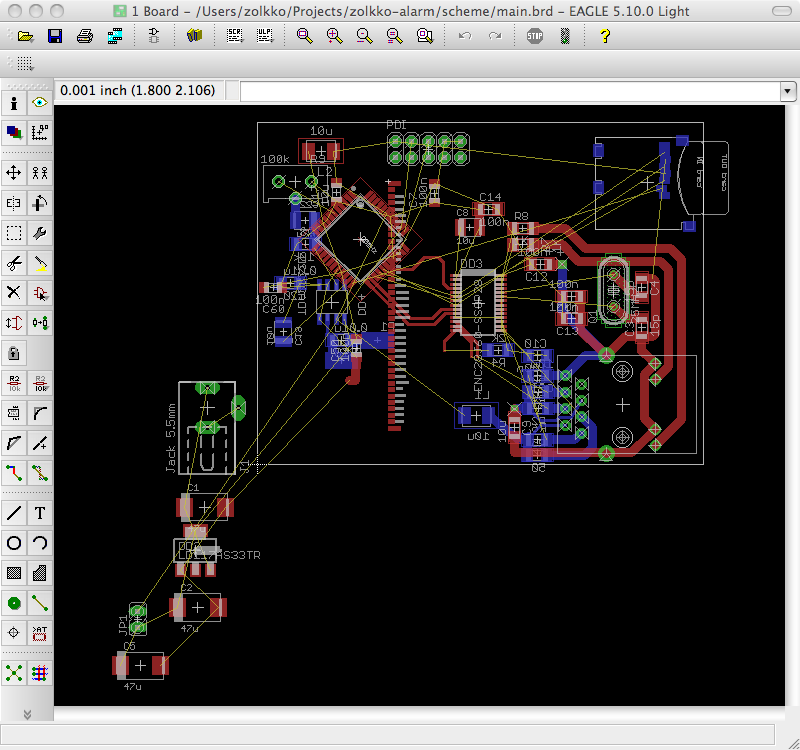
\includegraphics[bb=0 0 800 800, clip, scale=0.3]{eagle_brd.png}}
            \caption{Окно редактора печатных плат Eagle}
            \label{img:eagle_brd}
        \end{figure}

	
	\item{}Schematic Editor - программа для создания принципиальных электрических схем (рис. \ref{img:eagle_sch}).
		\begin{itemize}
			\item{}до 999 листов на одну схему;
			\item{}проверка эллектичских правил;
			\item{}обмен вентелей и пинов;
			\item{}возможность создания печатной платы из схемы одной командой.
		\end{itemize}
        \begin{figure}[h]
            \center{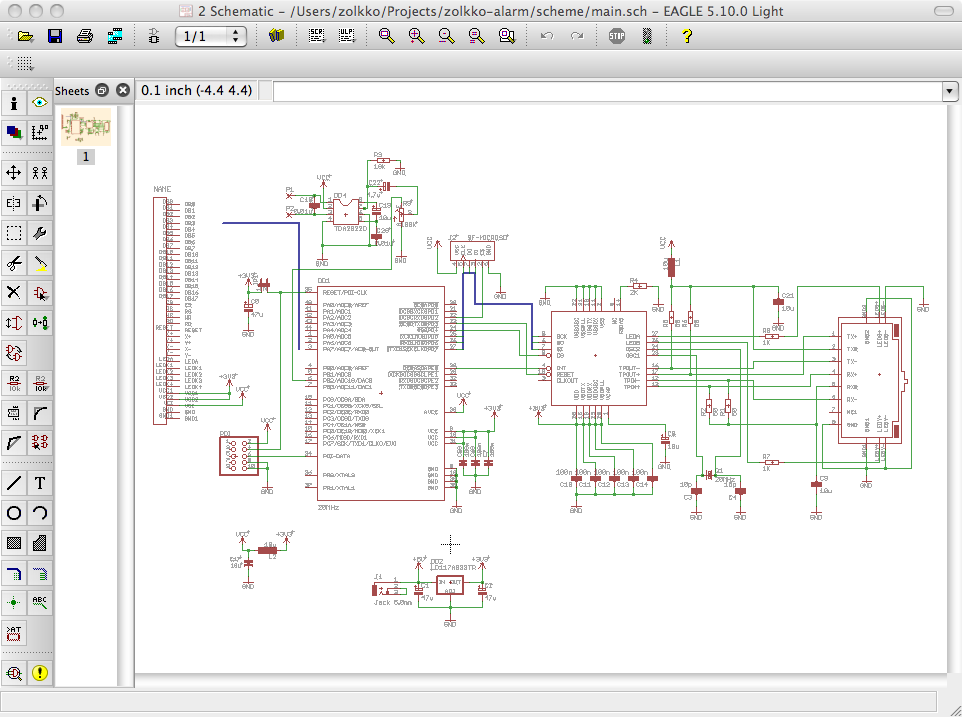
\includegraphics[bb=0 0 1010 730, clip, scale=0.3]{eagle_sch.png}}
            \caption{Окно редактора пренципиальных схем Eagle}
            \label{img:eagle_sch}
        \end{figure}
	\item{}Autorouter - программа автоматической трассировки.
		\begin{itemize}
			\item{}ripup-and-retry трассировщик - на первом проходе выполняется соединение абсолютно всех проводников без обращения внимания на возможные конфликты, заключающиеся в пересечении проводников на одном слое и нарушении зазоров. На каждом последующем проходе автотрассировщик пытается уменьшить количество конфликтов, разрывая и вновь прокладывая связи;
			\item{}до шестнадцати сигнальных слоёв;
			\item{}стратегия трассировки может быть подстроена заданием весовых коэфициентов.
		\end{itemize}
\end{enumerate}

Все эти программы встроены в один пользовательский интерфейс, таким образом нет необходимости в
предварительном конвертировании нет-листов.
\end{par}


\subsection{Обзор современных систем программирования микроконтроллеров}

Ведущими разработчиками 8/16 битных микроконтролеров на сегодняшний день
являются компании:
\begin{itemize}	
	\item{} Microchip Technology Inc. -- выпускающие микроконтроллеры семейства PIC и
		сигнальные микроконтроллеры dsPIC,
		получивших широкое распространение в странах серевной и южной америки.
		Отличительной особенностью PIC--контроллеров является хорошая преемственность
		различных семейств.
		8-битные микроконтроллеры представлены двумя базовыми архитектурами ядра:
		BASELINE и MID-RANGE. Основным инструментом разработки является среда программирования
		MPLab и набор компиляторов GCC.
	\item{} STMicroelectronics -- европейская компания, активно продвигающая свои 8 и 32
		разрядные микроконтроллеры на рынке. В качестве среды разработки предлагается
		использовать адаптированную версию набора компиляторов GCC.
	\item{} Texas Instruments --специализирующаяся на выпуске цифровых сигнальных процессоров
		и наиболее удачной линейки микроконтрллеров общего назначения MSP430.
	\item{} NXP Semiconductors -- производит 8 разрядные микроконтроллеры
			80C51: LPC900 и LPC700.
			Основным инструментом разработчика является адаптированная версия
			Keil PK51 Professional Developers Kit, предоставляющей инструменты для
			генерации программ для LPC, и включающая в себя среду разработки
			$\mu{}$Vision IDE, C51 ANSI C компилятор и A51 макро ассемблер, $\mu{}$Vision отладчик
			со встроенным симулятором ЦПУ и переферийных устройств. В комплект поставки
			среды так же входит внутрисхемный отладчик ISD51.			
	\item{} Freescale Semiconductor -- HC80, HC05, HC11.
	Эти микроконтроллеры используют расширенную архитектуру ЦПУ M68HC08.
	Основным иструментом разработки является CodeWarrior Development Studio, в поставку
	которой так же включается симулятор чипа и мастер автоматического генерирования
	кода ''Processor Expert''.
	\item{} Atmel Corporation -- выпускает микроконтроллеры AVR, основанные на ядре
	собственной разработки. Основное средство разработки -- AVR Studio. В начале 2011
	года компания прекратила поддержку старых версий AVR Studio 4 и AVR Studio 32,
	заместив их AVR Studio 5 -- средой разработки основанной на Microsoft Visual
	Studio Shell. В качестве компилатора выступает адаптированная версия GCC. Так
	же в комплекте среды разработки поставляется симулятор ЦПУ и переферии, и
	набор программного обеспечения ''AF''.
\end{itemize}

Таким образом, все лидирующие производители микроконтроллеров предоставляют
бесплатные системы программирования своих мкроконтроллеров.
Причём, можно отметить, что системы программирования либо основанны на коде 
набора компиляторов GNU GCC, либо в качестве стандартной среды разработки лицензируется
программное обеспечение других компаний. Во втором случае, зачастую, бесплатные
стандартные системы программирования обладают рядом ограничений, позволяющим только
опробовать демонстрационные проекты.

Однако, на рынке пристствует довольно большео число компаний специализирующихся
исключительно на создании систем программирования для встраиваемых систем. Лидером
в этой области является IAR Systems -- компания предоставляющая широчайший перечень компиляторов и стандартных библиотек для большого числа микроконтроллеров разных архитектур.
Их продукт IAR Embedded Workbench поддерживает следующие семейства микроконтроллеров:
\begin{itemize}
	\item{} 8051;
	\item{} ARM;
	\item{} Atmel AVR, AVR32;
	\item{} Freescale ColdFire, Freescale S08, Freescale HCS12;
	\item{} Maxim MAXQ;
	\item{} Microchip dsPIC/PIC24, PIC18;
	\item{} National CR16C;
	\item{} Renesas RL78, 78K, V850, H8, M16C, R8C, M32C, RX, R32C, SuperH;
	\item{} Samsung SAM8;
	\item{} STMicroelectronics STM8;
	\item{} TI MSP430.
\end{itemize}
Ещё одним интерестным продуктом этой компании является IAR visualState -- системе
программирования, автоматически генерирующей программный код на основе графически
заданного конечного автомата. При этом возможно проводить комдинированную разработку
программного обеспечения, когда часть кода программы генерируется автоматически, а часть
разрабатывается программистом.

\begin{figure}[h]
	\center{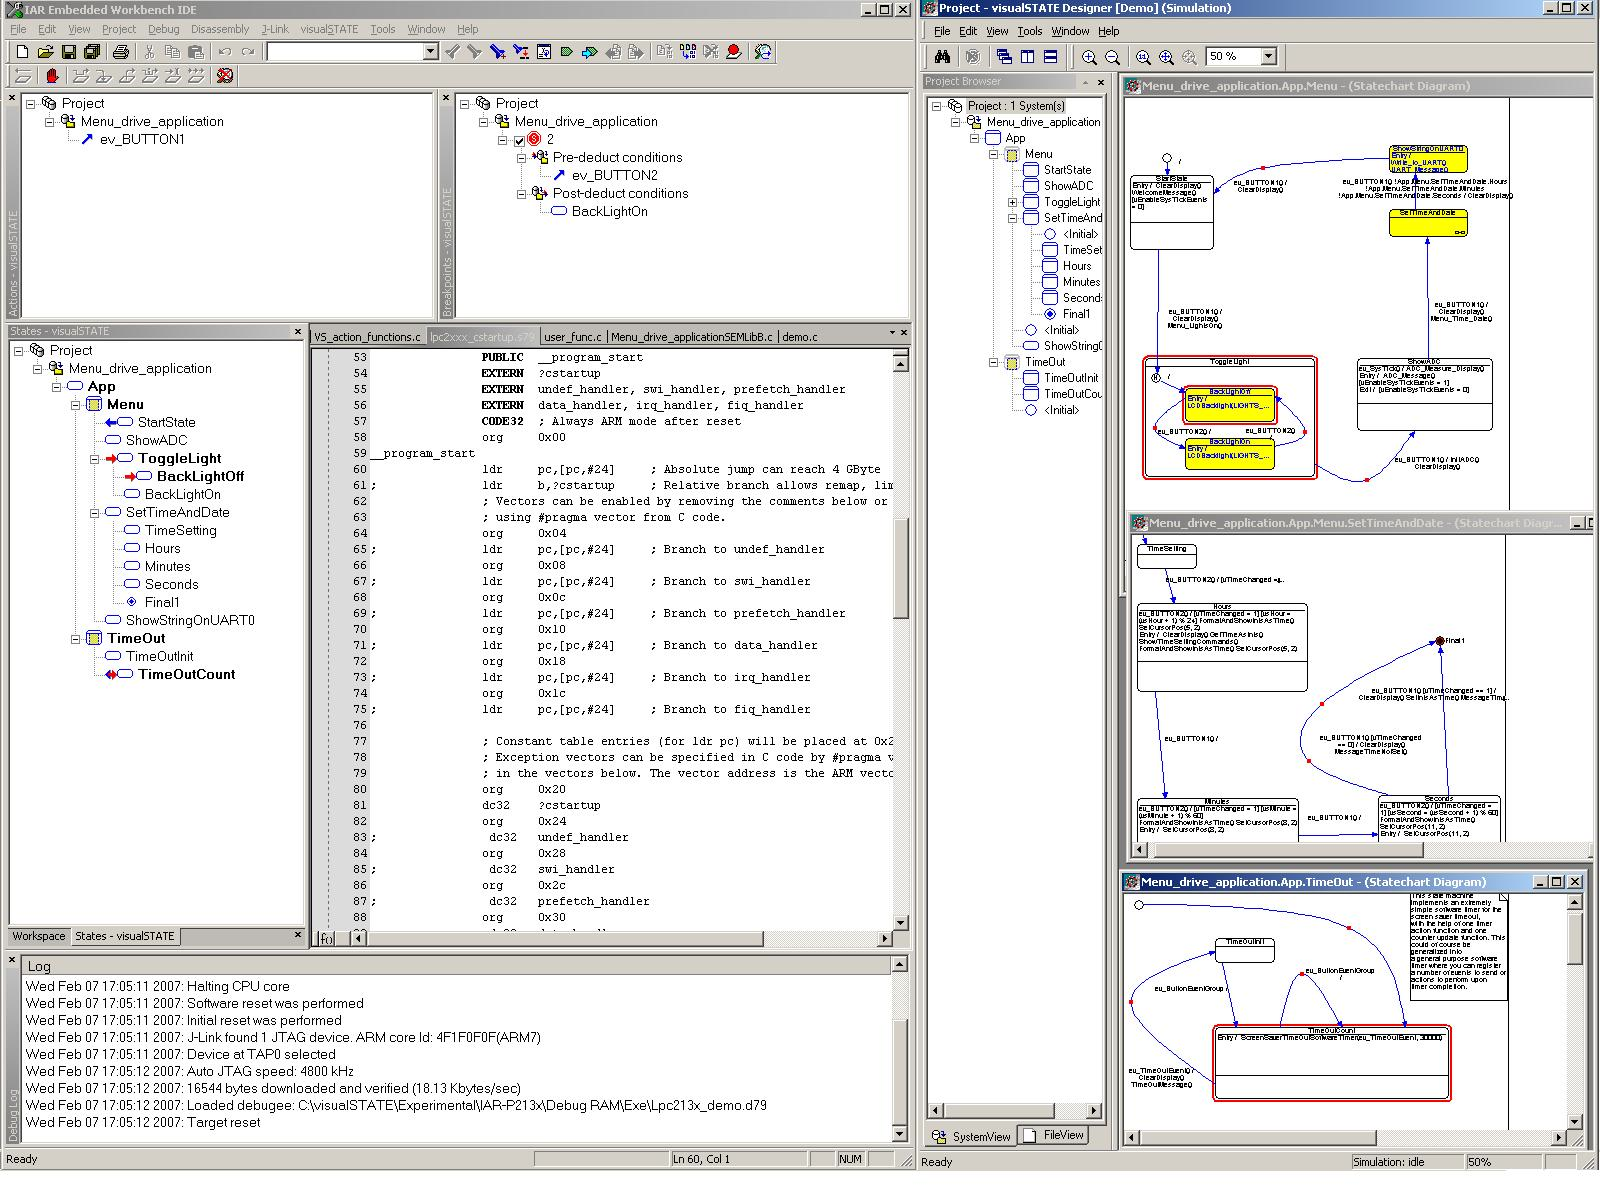
\includegraphics[bb=0 0 900 700, clip, scale=0.3]{iar_vis_state.png}}
	\caption{Среда разработки IAR visualSTATE}
	\label{img:iarVis}
\end{figure}

\newpage{}



%% Описываем выбор инструментария
%!TEX root = /Users/zolkko/Projects/zolkko-alarm/doc/main.tex
\section{Выбор инструментальных средств разработки микроконтроллерного программно-аппаратного комплекса}

\subsection{Выбор микроконтроллера}
Основными требованиями предъявляемыми мной к центральному вычислительному устройству
создаваемого устройства является:
\begin{itemize}
	\item{} невысокая стоимость;
	\item{} низкое энергопотребление;
	\item{} в число поддерживаемой переферии должен присутствовать ЦАП;
	\item{} аппаратная поддержка SPI;
	\item{} поддержка производителем этого рода устройств;
	\item{} доступность устройства;
	\item{} <<сильное>> сообщество разработчиков под эту архитектуру;
	\item{} наличие литературы и справочных материалов.
\end{itemize}


По всем этм пунктам идеально подходит микроконтрллер семейства XMega компании ATmel -- atxmega32a4.
Этот микроконтроллер полностью отвечает минимальным требованиям. В целях достижения максимальной
производительности и параллелизма у микроконтроллеров AVR используется
Гарвардская\\*
архитектура (рисунок \ref{img:avr_arch}) с отдельными памятью и шинами программ и данных. Инструкции,
хранящиеся в памяти программ, выполняются на одноуровневом конвейере. Это означает, что
во время выполнения одной инструкции выполняется предварительная выборка из памяти программ
следующей инструкции. Данная концепция делает возможным выполнение по одной инструкции за
каждый цикл синхронизации.

\begin{figure}[ht]
	\center{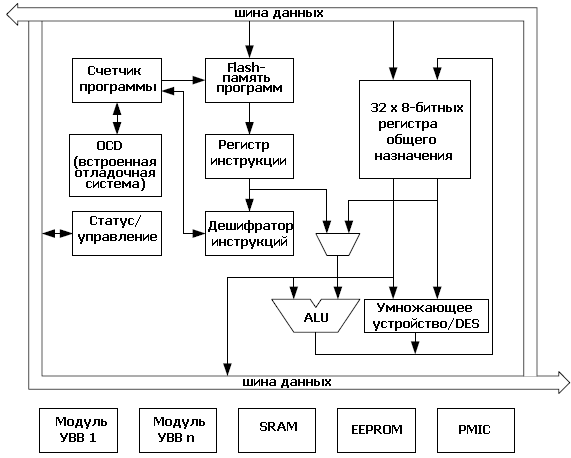
\includegraphics[bb=0 0 590 460, clip, scale=0.6]{avr_arch.png}}
	\caption{Архитектура AVR}
	\label{img:avr_arch}
\end{figure}


Так же в случае необходимости может быть заменён на более мощьный микроконтроллер того же семейства.
Для обеспечения этого функционала компания Atmel предприняла ряд шагов.

\begin{par}
    1. Была реорганизована область памяти, таким образом, чтобы все связанные между
            собой регистры располагались в памяти строго последовательно.
\end{par}
\begin{par}
    2. Была переписана стандартная библиотека C/C++, так чтобы обеспечивалась
            максимальная переносимость кода написанного для одного микроконтроллера
            на другой микроконтроллер того же семейства.
\end{par}

Микроконтроллеры серии XMega обладают следующими характеристиками:
\begin{itemize}
	\item{} 8/16-разрядное высокопроизводительное RISC ЦПУ AVR;
	\item{} 138 инструкций;
	\item{} аппаратное умножающее устройство;
	\item{} 32 8-битных регистра, напрямую подключенные к АЛУ
	\item{} прямая адресация до 16 Мбайт памяти программ и 16 Мбайт памяти данных;
	\item{} полная поддержка 16/24-битного доступа к 16/24-битным регистрам ввода-вывода;
	\item{} эффективная поддержка 8-, 16- и 32-битных арифметических инструкций;
	\item{} защита от изменения настроек критических функций системы.
\end{itemize}

Помимо этого, по сравнению с предыдущим семейством Mega \cite{avrref}, в микроконтроллеры семейства
XMega был внесен ряд значительных изменений.

\begin{par}
    1. Свехмалое энергопотребление обеспечиваемое технологией picoPower второго поколения.
    picoPower позволяет еще больше улучшить эффективность использования батарейного источника.
    То, что микроконтроллеры гарантируют нормальное функционирование при напряжении 1.6 В означает,
    что, например, в составе мобильных телефонов, они могут быть запитаны от стабилизированного
    источника напряжением 1.8В 10\%, тем самым, позволяя снизить себестоимость системы и увеличить
    длительность работы от батарейного источника. 
\end{par}

\begin{par}
    2. Event System -- позволяет организовать передачу данных между встроенными периферийными
    устройствами без вмешательства ЦПУ или использования ПДП.
    Этим гарантируется 100\% предсказуемость и малое время реагирования.
    До 8 одновременных событий или условий прерывания в периферийных устройствах могут автоматически
    инициировать действия в других периферийных устройствах \cite{avrxm}.
\end{par}

\begin{par}
    3. 12-разрядные АЦП и ЦАП. Для обеспечения высокоточной обработки аналоговых сигналов в состав 
    микроконтроллеров XMEGA интегрированы 12-битные преобразователи аналоговых сигналов. АЦП
    микроконтроллеров XMEGA могут достигать частоты преобразования до 2 МГц, что делает их самыми
	быстродействующими и точными на фоне АЦП обычных микроконтроллеров.
	Поскольку микроконтроллеры XMEGA также интегрируют два 12-битных ЦАП на частоту преобразования
	до 1 МГц и четыре усовершенствованных аналоговых компаратора, это делает их лидерами по
	степени интеграции компонентов для аналоговой обработки.
\end{par}

\begin{par}
   4. Расширена функциональность портов ввода-вывода общего назначения. Каждый из портов
    ввода-вывода может быть сконфигурирован как источник внешнего прерывания, при этом событие внешнего прерывания
    может минуюя ЦПУ запускать обработку данных используя модуль прямого доступа к памяти. \\*
    Новыми доступными состояниями портов ввода-вывода стали totem-pull, bus-keeper, wired-or, wired-and.
\end{par}


\subsection{Язык программирования микроконтроллера}
\begin{par}
Микропрограммы для микроконтроллеров XMega можно писать на нескольких языках программирования.
Сама компания Atmel предоставляет для программирования своих устройств два средства разработки:
	\begin{enumerate}
		\item{}AVR assembler -- язык низкого уровня, транслирует исходный код пользовательской
                программы в объектны и исполняемый код, его применение позволяет
                добиться от программы наибольшей производительности;
		\item{}AVR-GCC -- кодогенератор и набор дополнительных утилит для Gnu C Compiller от
                компании Atmel, активно поддерживаемый сообществом разработчиков, а так же
                входящий в комплект среды разработки AVR Studio, AVR32 Stdio и
                распростроняемый на правах свободного программного обеспечения, в состав
				которого входят компиляторы языка C и C++.
	\end{enumerate}
\end{par}

\begin{par}
В начале 2011 года компания предоставила новую версию своей интегрированной системы
разработки - AVR Studio 5. В отличии от предшественника, новая система позволяет разрабатывать
программное обеспечение для всех семейств микроконтроллеров AVR используюя единую среду разработки.
\end{par}

\begin{par}

\begin{figure}[ht]
	\center{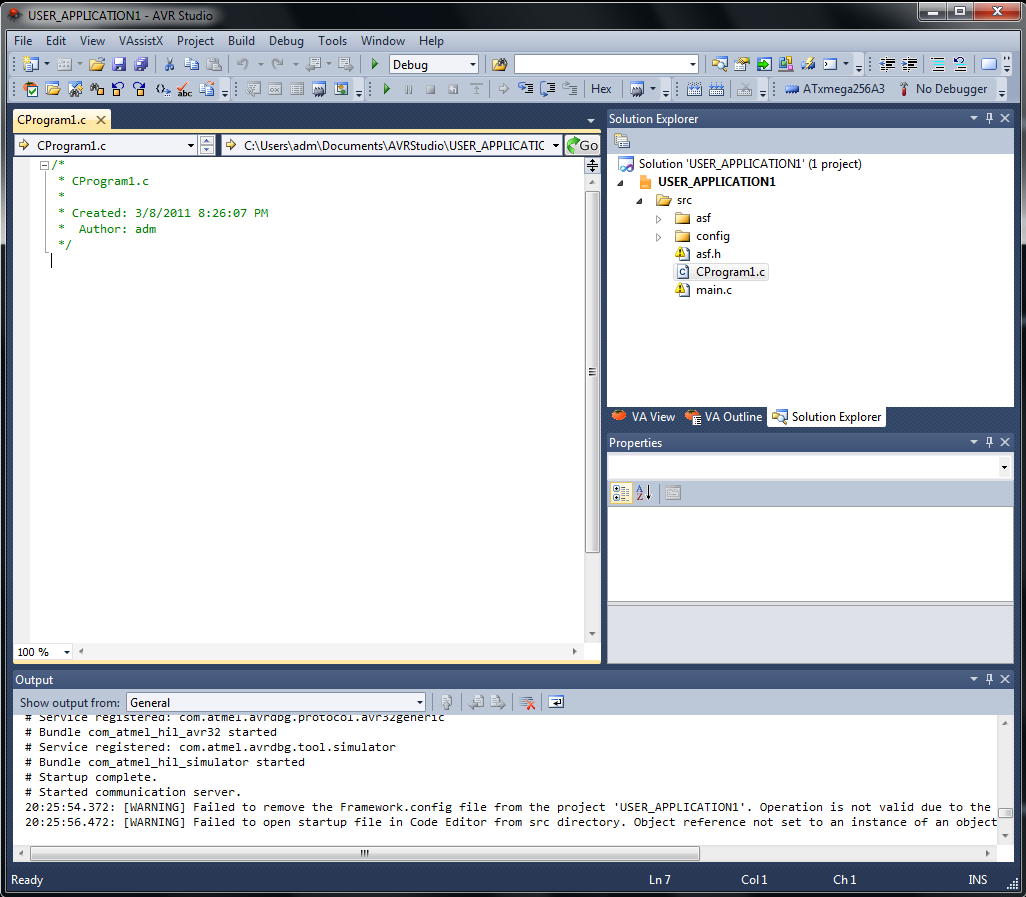
\includegraphics[bb=0 0 800 700, clip, scale=0.5]{avrstudio5.png}}
	\caption{AVR Studio 5}
	\label{img:avr_studio}
\end{figure}


Новая среда разработки AVR Studio 5 (рисунок \ref{img:avr_studio}) основана на базе лидирующего
продукта -- Microsoft Visual Studio.
И так же как и предшественники, новая версия AVR Studio 5  распространяется бесплатно.
В качестве компилятора и кодогенератора в AVR Studio 5 по прежнему используется AVR-GCC,
что позволяет продолжать использовать уже существующие наработки.
\end{par}

\begin{par}
Считается \cite{avrev}, что для разработки эффективного встраиваемого приложения для 8-битных микроконтрллеров
AVR наиболее целесообразно применять язык ассемблера или в случае, когда необходимо добиться
большей читаемости и поддерживаемости приложения -- язык С.
Однако, лидирующая группа японских производителей ЦПУ, возглавляемая NEC, Hitachi, Fujitsu и Toshiba,
разработала специализированных диалект языка C++ --- Embedded C++ (EC++), позволяющий применять
C++ для встраиваемых систем. Основная цель разработки --- перенос существующих методологий и шаблонов
программирования C++ в облать применения встраивамых систем.
При этом программы код генерируемых компиляторами EC++ может даже дать приемущества по сравлению
с языком C. Так как сама структура языка C++ позволяет минимизировать объём кода и одновременно
повышая его эффективность.
\end{par}

\begin{par}
Однако, при выборе в качестве языка программирования C++, из текущей реализации поставляемой с AVR-GCC,
необходимо учитывать некоторые её ограничения.
\end{par}

\begin{par}
 	1. В наборе компиляторов AVR-GCC отсутствует стандартная библиотека C++.
\end{par}

\begin{par}
	2. Необходимо помнить, что EC++ -- это только подмножество C++, по этому некоторые особенности языка были
        убраны из стандарта:
        \begin{itemize}
            \item{} множественное наследование;
            \item{} базовые виртульаные классы;
            \item{} информация времени исполнения;
            \item{} приведение типов (static\_cast, dynamic\_cast, reinterpret\_cast и const\_cast);
            \item{} квалификаторы типов;
            \item{} пространства имён;
            \item{} исключения;
            \item{} шаблоны.
        \end{itemize}
\end{par}



\subsection{Выбор языка программирования сетевого сервиса}

При проектировании сетевого сервиса от инструментального средства ожидается, чтобы оно
отвечало следующим требованиям \cite{technob}:

\begin{enumerate}
	\item{} инструментальное средство должно быть высокого уровня --- язык высокого уровня,
            освобождает разработчика от рутинной работы вроде ручного выделения и освобождения
            памяти, и позволяет ему сфокусироваться на оперировании абстракциями предметной области;

	\item{} язык должен минимизировать количество ошибок которые может допустить программист в
             процессе разработки системы;

	\item{} высокая степень параллелизма -- необходима возможность обслуживать тысячи клиентов
            одновременно;
	
	\item{} отказоустойчивость -- телеком-системы слишком масштабны, чтобы самому разработчику
             имело смысл даже пытаться предусмотреть все возможные ошибки;
	
	\item{} возможность обновления кода сервиса без останова выполнения программы;
	
	\item{} наличие обширной системной библиотеки,  а так же предопределённых каркасов
            проектов задающих общую структуру создаваемой системы, что позволяет ещё
            на этапе проектирования системы оценивать её будущие качества, а так же избавляет разработчика
			от необходимости реализовывать типовые решения самостоятельно, при этом тратя время на
			тестирование и отладку системы.
\end{enumerate}

\begin{par}
Один из немногих существующих и поддерживаемых на сегоднешний день языков программирования
отвечающих всем этим требованиям является Erlang и платформа Open Telecom Platform (OTP).
\end{par}

\subsubsection{Обзор языка Erlang и платформы OTP}

\begin{par}
В середине 1980-х, Ericsson Computer Science Laboratory было дано задание: исследовать языки
программирования подходящие для разработки телекоммуникационных продуктов нового поколения.
Джой Армстронг(Joe Armstrong), Роберт Вирдинг (Robert Virding) и Майк Вильямс (Mike Williams) под
руководством Брайна Декера (Bjarne Dacker) потратили два года на прототипирование
телекоммуникацинного приложения поочерёдно  используя все доступные на тот момент языки и
системы программирования. В результате, несмотря на то, что многие языки программирования обладали
интересными и подходящими свойствами, ни один из них не удовлетворял всех их требованиям. В результате
они приняли решение создать их собственный язык программирования.
\end{par}

\begin{par}
Erlang был создан под влиянием функциональных языков таких как  ML и Miranda, параллельных языков
ADA, Modula и Chill, и языка логического программирования Prolog. Erlang так же унаследовал некоторые
черты таких язков как Smalltalk, проприетарных языков Ericsson EriPascal и PLEX \cite{erlang}.
\end{par}

\begin{par}
Используя построенную на Prolog виртуальную машину Erlang (VM), лаборатория потратила  четыре года на
прототипирование телекоммуникационного приложения с применением и постоянными доработками новго языка.
Именно из-за применения метода проб и ошибок язык Erlang стал таким, каким он является сейчас. В 1999
Майк Вильямс переписал на Си виртуальную машину, и годом позже, на этом языке был выпущен первый
коммерческий продукт. 
\end{par}

\begin{par}
История создания языка Erlang важна для понимания его философии, так как в отличии от других языков,
которые находили свою нишу уже после разработки и распространения, Erlang изначально создавался
для решения конкретных задач бизнеса. Он создавался под задачи построения распределённых,
отказоустойчивых систем реального времени массового обслуживания.
\end{par}

\begin{par}
Так как такие области как системы поддержки продаж, банковские системы, системы компьютерной
телефонии, системы интеграции уровня предприятий зачастую предъявляют к своему программному
обеспечению аналогичные требования, то Erlang нашёл своё применение и в них.
\end{par}

Подтверждением применимости Erlang в этих областях могут служить факты использования этого языка в
проектах компаний:
\begin{itemize}
	\item{} Amazon -- использует Erlang для реализации SimpleDB, предоставления системы
        управления базами данных как части Amazon Elastic Compute Cloud (EC2);
	\item{} Yahoo! -- использует Erlang для реализации своего сервиса социальных закладок,
    который обслуживает более 5 милионов пользователей и 150 милионов URL;
	\item{} T-Mobile -- использует Erlang в их SMS и авторизирующей системах;
	\item{} Motorola -- использует Erlang в системе обработки звонков системы обслуживания клиентов;
	\item{} Ericsson -- использует Erlang для поддержки узлов используемых в GPRS и 3G
    мобильных сетях по всему миру;
	\item{} Facebook и Yandex -- используют написанный на Erlang сервер мгновенных
    сообщений Ejabberd.
\end{itemize}


%%\section[Детализация постановки задачи]{ДЕТАЛИЗАЦИЯ ПОСТНОВКИ ЗАДАЧИ}
\section{ДЕТАЛИЗАЦИЯ ПОСТАНОВКИ ЗАДАЧИ}
\begin{par}
Целью выполняемой работы является автоматизированное проектирование программно-аппаратного комплекса
на основе микроконтролера AVR семейства XMega --- atxmega32a4, позволяющего учитывать текущее время
и выдавать сигнал звукового оповещения при достижении времени заданного пользователем устройства.
\end{par}

\subsection{Функциональная структура устройства}

Функциональная структура устройства приведена на рисунке \ref{img:funcd}.

\begin{figure}[h]
	\center{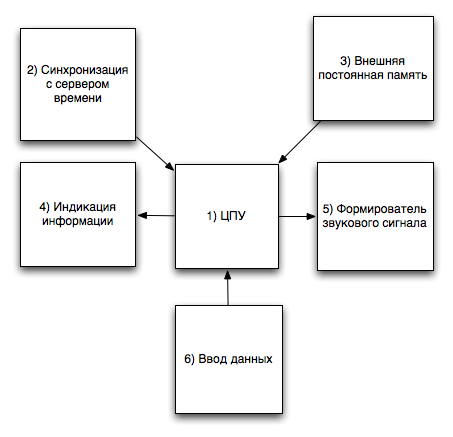
\includegraphics[bb=0 0 453 437, clip, scale=0.8]{funcd.png}}
	\caption{Фнкциональная структура}
	\label{img:funcd}
\end{figure}

\begin{enumerate}
    \item{}ЦПУ --- основной блок отвечает за отсчёт врени и за организацию канала коммуникации
        между блоками воспроизведения мелодии, хранения данных мелодии, и модуля синхронизации времени.
    \item{}Модуль синхронизации времени отвечает за получение информации о текущем веремни
            от удалённого SNTP сервера.
    \item{}Модуль постоянной памяти отвечает за хранение данных, используемых для формирования
        мелодии будильника.
    \item{}Модуль индикации отвечает за отображение текущего времени и наступившего события
        будильника.
    \item{}Модуль формирования аналогово сигнала иcпользуется для формирования сигнала и проигрывания
            мелодии будильника.
    \item{}Модуль ввода данных используется для устновки текущего времени и задания
        времени срабатывания будильника.
\end{enumerate}


\subsection{Описание работы устройства}
\subsubsection{Центральный микроконтроллер}
\begin{par}
Центральное место в схеме занимает микроконтроллер atxmega32a4. Микропрограмма контроллера
должна быть составлена таким образом, что бы прерывание модуля RTC происходило с частотой 2 Гц.
При приходе прерывания микроконтроллер отсчитывает количество $ \frac{1}{2} $ с. прошедших с момента
включения схемы и выводит текущее время на устройство индикации.
\end{par}

\begin{par}
Программа микроконтроллера должна быть написана на языке C++ для компилятора входящего в поставку
AVR-GCC, с учётом всех допущений указанных в разделе <<Язык программирования микроконтроллра>>.
\end{par}

\subsubsection{Устройство индикации}
\begin{par}
В качестве устройства индикации должен использоваться TFT ЖК-дисплей DST2001PH\cite{display} со встроенным
драйвером ili9320 включённым в режиме system i80 16-бит\cite{ili9320}.
Так как количество портов\\*
ввода-вывода на используемом микроконтролере достаточно, введение дополнительных узлов
расширяющих возможности 
ввода-вывода микроконтроллера --- не предусматривается.
\begin{figure}[h]
	\center{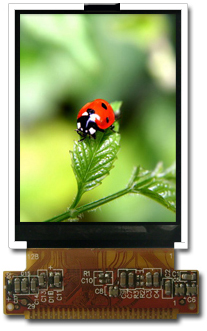
\includegraphics[bb=0 0 150 250, clip, scale=1.0]{ili9320.png}}
	\caption{Внешний вид TFT ЖК-дисплея DST2001PH}
	\label{img:iili9320}
\end{figure}
\end{par}



\begin{par}
В начальный момент работы, устройство должно погасить изображение на ЖК-дисплее и подготовить внутреннюю
память модуля индикации.
\end{par}

\subsubsection{Ввод данных}
\begin{par}
Модуль ввода данных пользователя должен быть выполнен на сенсорном экране ЖК-дисплея,
выполненного по 4-проводной схеме включения резистивного сенсорного экрана. Для
оцифровки значений плучаемых с сенсорного экрана должны использоваться АЦП\cite{avradc} центрального
микроконтроллера.
\end{par}

\begin{par}
В начальный момент работы устройства, после инициализация внутренней памяти ЖК-дисплея, должна быть
произведена процедура калибровки сенсорного экрана, а полученные коэффициенты далее должны быть
использованы для корректировки показаний снятых с сенсорного экрана. Это позволит отказаться
от дополнительной схемы температурной компенсации и статических калибровочных показателей,
и при этом устройство будет выдавать давольно стабильный результат,
так как эксплуатироваться устройство будет в условиях постоянной комнатной температуры,
а собственная рассеиваемая мощьность устройства не должна быть велика на столько, что бы
вносить ощутимую погрешность в показания.
\end{par}


\subsubsection{Звуковое оповещение о наступившем событии}
\begin{par}
Звуковое оповещение о наступившем событии должно быть выполнено на широко распростонённой
микросхеме mc34119, включённой в стандартном режиме (рис. \ref{img:mc34119m}).
\begin{figure}[h]
	\center{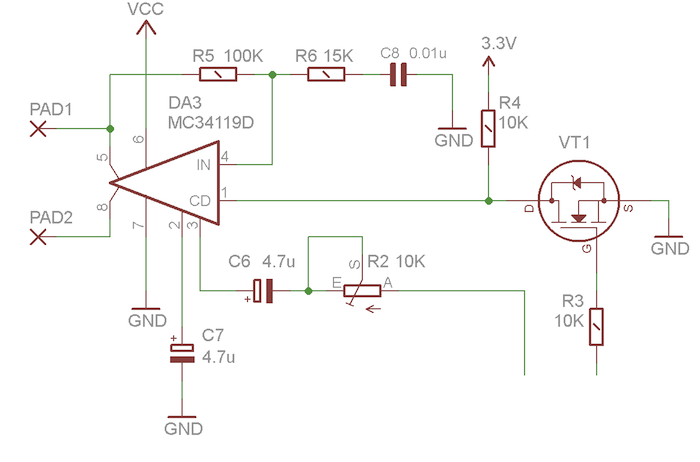
\includegraphics[bb=0 0 200 190, clip, scale=0.8]{mc34119.png}}
	\caption{Схема включения mc34119}
	\label{img:mc34119m}
\end{figure}
\end{par}

\begin{par}
В начальном состоянии на вход Chip Disable микросхемы mc34119 должен подаваться сигнал высокого уровня.
Это переводит микросхему в состояние низкого энергопотребления \cite{mc34119}.
\end{par}

\begin{par}
В момент наступления события будильника на вход Chip Disable микросхемы необходимо подать сигнал 
низкого уровня, выполнить задержку не менее 40 мс., необходимую для перевода микросхемы в
нормальное состояние, и затем подавать на неё вход сигнал с ЦАП центрального микроконтроллера.
Принципиальная схема ЦАП микроконтроллеров AVR семейства XMega приведена на рисунке \ref{img:avrdacp}.
\begin{figure}[h]
	\center{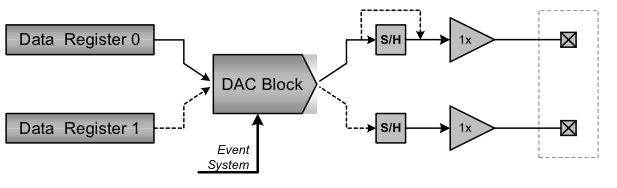
\includegraphics[bb=0 0 300 100, clip, scale=0.8]{avrdac.png}}
	\caption{Принципиальная схема ЦАП микроконтроллеров AVR семейства XMega}
	\label{img:avrdacp}
\end{figure}
\end{par}

\begin{par}
Для воспроизведения музыкального отрывка необходимо использовать нижние 8 бит 12-битного
ЦАП микроконтроллера. Опорное напряжение ЦАП микроконтроллера должно быть равно либо внутреннему
напряжению микроконтроллера 1 В, либо стабилизированному напряжению питания ($AV_{cc}$). Выбор того или иного
опорного напряжения ЦАП обусловливается параметрами динамика и необходимым уровнем громкости.
Для переодического получения данных и их переноса в буфер воспроизведения необходимо использовать
обработик прерывания таймера Timer 1 микроконтроллера. Частота срабатывания таймера выбирается
в соответствии с частотой дискретизации музыкального отрывка.
Механизм программирования ЦАП микроконтроллеров AVR семейства XMega детально описан в документации\cite{avrdac}.
\end{par}


\subsubsection{Устройство хранеия музыкальных отрывков}
\begin{par}
В качестве устройства хранения звуковых отрывков необходимо использовать энергонезависимые карты
памяти MicroSD. Применение этого вида памяти позволит не пребегая к перепрограммированию устройства
вносить музыкальные фрагменты на карту с персонального компьютера, оснащённого модулем
чтения/записи карт MicroSD.
\end{par}

\begin{par}
Для воспроизведения звуковых отрывков центральным микроконтроллером должен быть
организован буфер воспроизведения, таким образом, что бы в случае отсутствия карты MicroSD или
сбоя доступа к ней, в него вносились записанные на этапе программирования данные EEPROM микроконтроллера.
\end{par}

\begin{par}
Для чтения данных карт памяти MicroSD должен использоваться SPI режим работы. Методика программирования
интерфейса SPI микроконтроллеров AVR семейства XMega дана в документации \cite{avrspi}.
\end{par}

\subsubsection{Синхронизация времени}
\begin{par}
В качестве контроллера сетевого интерфейса необходимо использовать микроконтроллер фирмы Micro Chip
enc28j60. Пример включения этого микроконтроллера дан на рисунке \ref{img:ienc28j60}.
\begin{figure}[h]
	\center{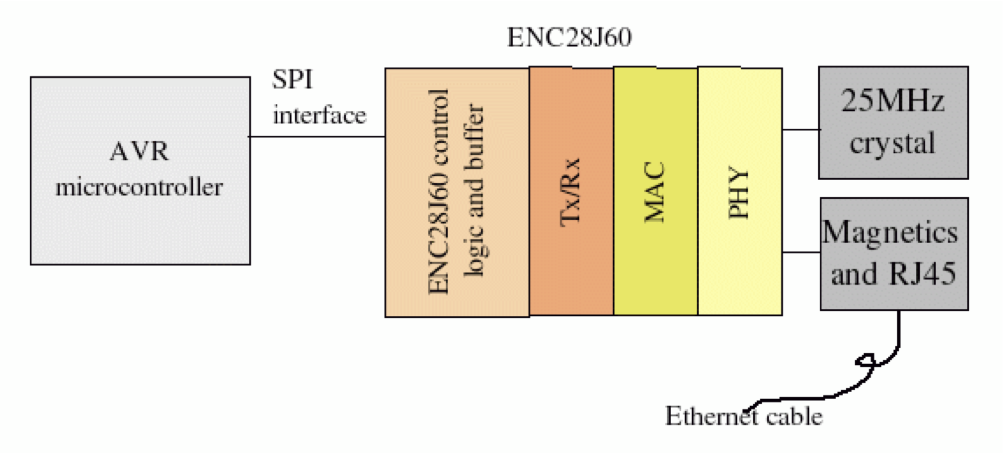
\includegraphics[bb=0 0 500 220, clip, scale=0.6]{enc28j60.png}}
	\caption{Схема включения микроконтроллера enc28j60}
	\label{img:ienc28j60}
\end{figure}

Этот микроконтроллер требует использования трансформатора с отношением 1:1 сертефицированного
для сетей 10base-T. По этому для упрощения изделия необходимо использовать готовые RJ45
коннекторы ''Magjack'', которые включают в своей конструкции необходимые трансформаторы и
свето диоды. В случае использования этого метода в схему устройства необходимо будет добавить
только одну индуктивность в 10 мкГн.
\end{par}

\begin{par}
Один раз в 30 минут устройство должно повышать рабочую частоту микроконтроллера до 32 МГц.
И производить попытку синхронизации времени с удалённым SNTP сервисов. По завершению процедуры
синхронизации времени, устройство должно вновь перевести микроконтроллер на рабочую частоту 2 МГц.
\end{par}

\begin{par}
Взаимодействие центрального микроконтроллера и микроконтроллера сетевого интерфейса осуществляется
по протоколу SPI \cite{enc28j60}, расширенному дополнительными сигнальными линиями.
\end{par}


\subsection{Проектирование принципиальной схемы и печатной платы}
\begin{par}
Необходимо разработать принципиальную схему и печатную плату устройства в системе автоматизированного
проектирования Eagle.
\end{par}

\begin{par}
Необходимо разработать схемотическое обозначение и посадочное мето для подключения ЖК-дисплея.
\end{par}

\begin{par}
Необходимо провести DRC проверку выполненой печатной платы на соотвествие параметрам:
\begin{itemize}
    \item{} Количество слоев: до 2;
    \item{} максимальный размер платы (размер рабочего поля): 380х320 мм;
    \item{} минимальная ширина проводника/минимальный зазор: 0,24/0,24 мм;
    \item{} минимальный отступ полигона: 0,24 мм;
    \item{} минимальный диаметр отверстия/минимальная площадка на переходном отверстии: 0,2/0,6 мм;
    \item{} минимальной диаметр монтажного отверстия — 0,6 мм;
    \item{} размер минимальной контактной площадки: для металлизированных отверстий 1,2—1,6 мм — +0,55 мм;
    \item{} минимальная толщина линии шелкографии (маски) — 0,15 мм;
    \item{} минимально допустимое отторжение маски от КП — 0,1 мм, для КП ИМС с шагом 0,5 мм — 50 мкм;
    \item{} минимальная высота шрифта шелкографии — 1,5 мм.
\end{itemize}
\end{par}

\subsection{Разработка SNTP сервиса}
\begin{par}
Необходимо разработать SNTP сервис на языке ErLang. Дополнительных требований к проектированию этого сервиса
не предъявляется, так как основное его назначение --- получение более удобного
инструмента отладки подпрограммы синхронизации времени.
При этом делается допущение, что успешный результат испытания по синхронизации свремени с разрабатываемым
сервисом, подтверждает правильность работы как самого сервиса, так и микропрограммы устройства.
\end{par}
\newpage{}

\section{Организационно-экономическая часть}

\subsection{Описание разрабатываемого продукта}
\begin{par}
Разработанное устройство --- <<цифровые часы с будильником>> позволяют отображать
текущее время на большём графическом жидкокристалическом дисплее. Удобным для
потребителя методом производить ввод времени срабатывания будильника.
Устройство позволяет не пребегая к перепрограммированию внутренней памяти менять
мелодию звуковой сигнализации. А так же производить синхронизацию текущего времени
с высокоточным удалённым сервером времени.
\end{par}

\begin{par}
К достоинству системы так же можно отнести то, что она реализована в соотвествии с манифестом
разработчиков открытого аппаратного обеспечения, что может прозволит повысить качество потребительских
характеристик устройства за счёт привлечения сообщества разработчиков открытого аппаратного
обеспечения. Так устройство или его часть может быть использовано в других ещё более
совершенных бытовых устройствах разрабатываемых сторонними производителями.

\begin{figure}[h]
	\center{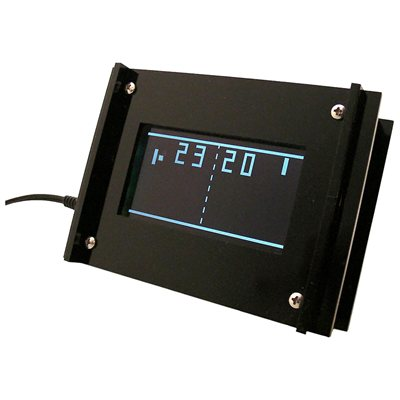
\includegraphics[bb=0 0 300 300, clip, scale=0.8]{adafruit.png}}
	\caption{Adafruit Monochron Open Source Clock kit}
	\label{img:adafruit}
\end{figure}

\end{par}

\subsection{Исследование существующих программных продуктов}
\begin{par}
Фактически на текущий момент на рынке существует только один аналог разработанного
утройства ---  Adafruit Monochron Open Source Clock kit.
Сравнительный обзор устройств представлен в таблице \ref{table:compare}.
\end{par}


\begin{par}
\begin{table}
\caption{Сравнение ''Цифровые часы с будильником'' и ''Adafruit''}
\begin{tabular}{|l|p{4cm}|p{4cm}|}
\hline{}
Характеристика & Цифровые часы с\linebreak{} будильником & Adafruit \\
\hline{}
Микроконтроллер & новое поколение AVR Xmega --- atxmega32a4 & старое семейство контроллеров AVR Mega -- atmega328 \\
\hline{}
ЖКИ & TFT 320x240 & LCD 128x64 \\
\hline{}
Метод ввода & сенсорный экран & кнопочное управление \\
\hline{}
Мелодии будильника & разнообразные мелодии выбираемые пользователем, одна встроенная мелодия & мерцание ЖКИ и звуковая сигнализация пъезоэлектрическим излучателем \\
\hline{}
Синхронизация с сервером времени & присутствует & отсутствует \\
\hline{}
Количество вариантов сборки & 1 & более 10 \\
\hline{}
Ориентировочная цена & 90\$ & 90\$ \\ 
\hline{}
Привлекательное название & отсутствует & присутствует \\ 
\hline
\end{tabular}
\label{table:compare}
\end{table}

Как видно из представленной таблицы, спректированное устройство имеет ряд преимуществт перед
устройством Adafruit. К недостаткам можно отнести только низкое число вариантов сборки устройства,
вызванное малой распространённостью разработанного устройства, что является
следствием не завершёности стадии его проектирования и разработки, а так же отстутствием каких-либо
действий нацеленных на устронение этого недостатка.
\end{par}
\newpage{}


%%\section{Разработка программно-аппаратного комплекса}
%%Расчёт органичивающего ток резистра светодиодной подсветки ЖКИ DST2001PH

\begin{par}
В данном ГЖКИ используются четыре параллельно соединённых светодиода белого свечения со следующими характеристиками:
\begin{itemize}
    \item{}Допустимый ток --- 15мА
    \item{}Прямое падение напряжения --- 3.2В
\end{itemize}

Таким образом ограничивающий ток резистор должен иметь сопротивление не менее: \\
$$R = (U_n - U_p) / I$$ \\
$$R = (3.3 - 3.2) / 0.015 = 6.6$$ \\
Ближайшее значение стандартного резистра будет 6.8Ом.

\end{par}


Управление яркостью светодиодов подсветки ЖКИ производиться методом широтно-импульсной модуляции.

%%\subsection{Управление яркостью светодиодной подсветки ЖКИ}

\begin{par}
Одним из основных параметров светодиодов является: яркость — величина,
равная отношению силы света к площади светящейся
поверхности, измеряемая в канделах на квадратный метр. \\

Спектральная характеристика светодиода выражает зависимость интенсивности
излучения от длины волны излучаемого света и дает представление о цвете
свечения светодиода. \\

Длина волны излучаемого света определяется разностью
энергий двух энергетических уровней, между которыми происходит переход
электронов на излучательном этапе процесса рекомбинации и определяется
исходным полупроводниковым материалом и легирующими примесями.
\end{par}

\subsubsection{Уменьшение яркости светодиода методом ШИМ}

\begin{par}
Наиболее простой способ уменьшения яркости светодиода - изменение прямого
тока или напряжения [http://www.e-neon.ru/user_img/pages/Dimming_InGaN_rus.pdf].
Но необходимо учитывать, что изменение этих параметров будет влиять на
длину волны излучаемого света, причём чем больше длинна волны, тем сильнее
выражен этот эффект.
Помимо тока, на длину волны оказывает влияние так же и температура.
Но это влияние не столь существенно и может игнорироваться.
\end{par}

\begin{par}
В схемах с использованием ШИМ через светодиод проходит последовательность импульсов.
Если частота следования импульсов более 200Гц, человеческий
глаз, обладающий инерционностью[TODO], будет ощущать непрерывное свечение
светодиода. Изменняя длительность и скважность импульса можно добиться того,
что зрение будет интегрировать и интерпретировать отдельные световые импульсы
как изменение силы света.
\end{par}

\begin{figure}[h]
	\center{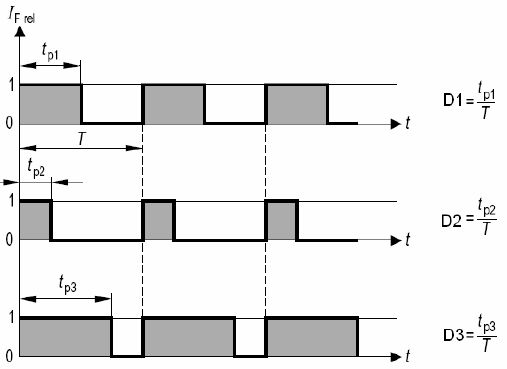
\includegraphics[bb=0 0 507 396]{led_pwm.png}}
	\caption{Управление яркосьтю светодиода ШИМ}
	\label{img:led_pwm}
\end{figure}

\begin{par}
При неизменном токе яркость свечения зависит от скважности
следующим образом: \\
    $$ D_2 < D_1 < D_3 $$

При этом, визуальная сила света будет меняться линейно при соответствующем
линейгном изменении скважности [TODO: откуда я взял эту информацию].
\end{par}

[TODO: А так же какова будет зависимость в чиселках]



%% Библиография
\renewcommand{\refname}{СПИСОК ЛИТЕРАТУРЫ}

\begin{thebibliography}{99}
\bibitem{lessing} Lawrence Lessig. ''Free culture: how big media uses technology and the law to lock down
culture and control creativity'', ''Rebuilding Free Culture: One Idea'', KF2979.L47, с. 345
\bibitem{electric} http://www.staticfreesoft.com/electric.html
\bibitem{geda} http://en.wikipedia.org/wiki/Geda
\bibitem{avrref} Atmel corp., ''XMEGA A MANUAL'', с. 433
\bibitem{avrxm} http://atxmega.narod.ru/, структурное описание, 
\bibitem{avrev} Евстифеев А.В. ''Микроконтроллеры AVR семейства Mega''., М.: Додэка-XXI, 2007, с. 587
\bibitem{technob} Одинцов В., ''Профессиональное программирование. Системный подход. 2 изд.'', BHV-СПб 2006, с. 405
\bibitem{erlang} Francesco Cesarini, Simon Thompson, ''Erlang Programming'', 2009, с. 470
\bibitem{display} Displaysun, ''Specification for TFT LCD module DST2001PH'', DST2001PH REV B, 2008/02/23, с. 24
\bibitem{ili9320} ILITek., ''a-Si TFT LCD Single Chip Driver 240RGBx320 Resolution and 16.7M color'', с. 115
\bibitem{avradc} Atmel corp., ''AVR1300: Using the XMEGA ADC'', Rev. 8033B-AVR-04/08, с. 6
\bibitem{mc34119} Freescale Semiconductor, ''Low power audio amplifier 34119. Technical Data.'', Rev. 3.0, 12/2006, с. 16
\bibitem{avrdac} Atmel corp., ''AVR1301: Using the XMEGA DAC'', Rev. 8033B-AVR-04/08, с. 8
\bibitem{avrspi} Atmel corp., ''AVR1309: Using the XMEGA SPI'', Rev. 8057A-AVR-02/08, с. 6
\bibitem{enc28j60} Microchip inc., ''ENC28J60 Data Sheet. Stand-Alone Ethernet Controller with SPI Interface'', с. 93
\end{thebibliography}
\end{document}

